%!TEX root = main.tex

\section{Analysis of Web Search Flows}
\label{sec:web_search}

\begin{figure}[th]
\centering
	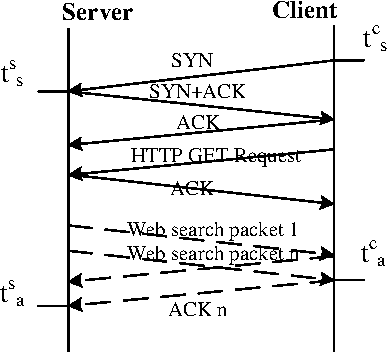
\includegraphics[width=0.5\linewidth]{web_finish_time_example}
\caption{Time-line in web search flow.}
\label{fig:web_finish_time_example}
\end{figure}

Web search starts when mobile terminal initiates connection to transmit query text, and ends when server receives acknowledgments of all search content. Figure~\ref{fig:web_finish_time_example} shows the typical time-line in web search flows. In web search, user-perceived latency is the duration from transmitting SYN packet to receiving all web search data, \ie $t^c_a - t^c_s$. Yet we could not obtain these two timestamps at server side when collecting dataset. Alternatively, we use the duration $t^s_a - t^s_s$ to approximate the latency that user perceives, \ie from that server transmits SYN-ACK packet, to that server receives all acknowledgments. This is also how \emph{finish time} in web search is defined.

\begin{figure}[th]
\centering
	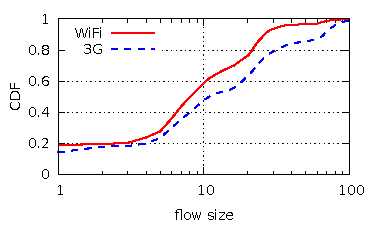
\includegraphics[width=0.8\linewidth]{web_flow_size}
\caption{The distribution of flow sizes in web search.}
\label{fig:web_flow_size}
\end{figure}

In this section, we first study the impact of flow size on finish time in web search flows. Figure~\ref{fig:web_flow_size} shows the distribution of flow sizes in web search.  From the figure, all flows are with less than 100 data packets, in which a large fraction of flows are with size in range between 4 and 30 packets. There are also flows with no search result, resulting in one data packet in the flow, which occupy 15\% of flows. The median value of flow size in WiFi network is smaller than that of flows in 2G/3G network. Mobile terminals in cellular network are more likely to do intentioned search, like route to the destination, weather condition. On the other hand, mobile terminal in WiFi network are more likely to do random search, like information of celebrity, sport news. This may help to explain the difference of flow size in different networks.

The flow size in web search ranges from 1 to 100 packets. This means that the data could be transmitted in 1 RTT at least, and more than 4 RTT at most. Considering the various flow sizes, the metric $finish\_time$ could not portray the efficiency that the data is delivered. To eliminate the affect of flow size, we introduce one more performance metric transmission time per packet ($tpp$), defined as the average time to transmit a data packet. The metric $tpp$ could be represented as $\frac{finish\_time}{\#(pkts)}$. In the following, we mainly use transmission time per packet ($tpp$) to depict the performance of web search.

\subsection{Impact of TCP state}

Next, we divide the analysis of web search flow into 3 different pieces corresponding to the three subsequent stages: \emph{3-way handshake}, \emph{slow start}, \emph{congestion avoidance}, and investigate the impact on finish time separately in different stages.

In TCP 3-way handshake, server establishes connection with client, in preparation for data transmission. Ideally, this stage completes in 1 RTT. However, in the dataset we could see that a non-negligible fraction of flows experience SYN retransmission in 3-way handshake. In slow start stage, server does not encounter packet loss or reordering event. Thus it enlarges the congestion window by 1 segment size for each received acknowledgment, and transmits data constrained by the window size. Server leaves slow start and enters congestion avoidance stage when it encounters congestion event, like packet loss. In congestion avoidance stage, server reduces the congestion window when detecting packet loss through fast retransmit\cite{jacobson1988congestion} and compels the congestion window to grow from 1 segment size when detecting packet loss through RTO. Slow start and congestion avoidance stages constitute data transmission. It is worth noting that, different from the TCP congestion avoidance state in TCP/IP stack, the \emph{congestion avoidance} stage here starts when server detects congestion event and ends till the flow finishes. 

\begin{figure}[th]
\centering
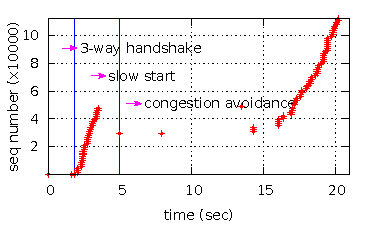
\includegraphics[width=0.8\linewidth]{web_three_stages}
\caption{The three stages in web search flows.}
\label{fig:web_three_stages}
\end{figure}

The three stages could be exemplified in Figure~\ref{fig:web_three_stages}, which shows the time-line and sequence number of a real flow in web search. In the figure, server takes 1.8s to establish connection, 3.1s to transmit 35 data packets in slow start stage, and 15.3s to transmit the left 48 data packets in congestion avoidance stage. In the following, we use the criteria of partitioning to break the analysis down into the three stages that flows experience.

\subsubsection{3-Way HandShake}
\begin{figure}[th]
\centering
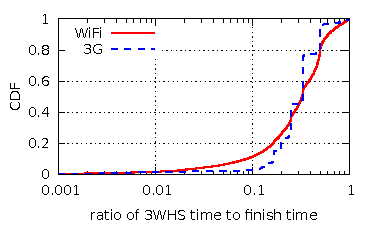
\includegraphics[width=0.8\linewidth]{web_handshake_time_ratio}
\caption{The ratio of time in 3-way handshake to finish time in each flow.}
\label{fig:web_handshake_ratio}
\end{figure}

In Figure~\ref{fig:web_handshake_ratio}, we plot the ratio of time consumed by 3WSH (3-Way HandShake) to the finish time. From the figure, flows in cellular network have similar ratio of time in 3-way handshake to that in WiFi network (with median value 0.3). If the 3WSH could be removed from finish time, the user-perceived web search latency would be reduced by 30\% in more than half of the flows. Moreover, there are 8\% of flows in WiFi network consuming 70\% of their time in 3WSH.

The unexpectedly high ratio of 3WSH could be introduced by two reasons. First, most of web search flows contains packets ranging from 1 to 100, these data could transmitted in 1 to 4 RTT's if there is no congestion event. Thus 3WHS, without transmitting any data, occupies a large fraction of time in short flows. Second, there are a non-negligible fraction of flows experiencing SYN retransmission during 3WHS stage. Table~\ref{tab:web_syn_retrans} illustrates the percentage of flows with SYN retransmission. In the table, 4.4\% of flows in WiFi network also suffer from timeout retransmission in 3WSH, which takes 1 second (\ie the initial RTO) to retransmit the SYN packet. One way to mitigate the costly 3WSH in short flows is to maintaining TCP connections before user demands web requests.

\begin{table}[th]
\centering
\renewcommand{\arraystretch}{1.1}
\caption{Percentage of flows that experience SYN retransmission in web search.}
\label{tab:web_syn_retrans}
\begin{tabular}{l|c|c|c}
\toprule
& WiFi & 2G & 3G \\
\midrule
SYN retransmission & 4.4\% & 2\% & 0.5\% \\
\bottomrule
\end{tabular}
\end{table}

\subsubsection{Slow Start stage}
\begin{figure}[th]
\centering
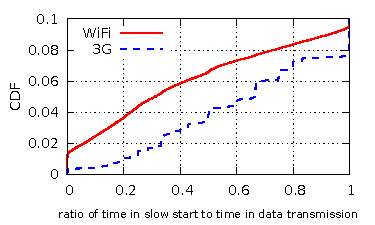
\includegraphics[width=0.8\linewidth]{web_slowstart_time_ratio}
\caption{The ratio of time in slow start to the time in data transmission.}
\label{fig:web_ss_time_ratio}
\end{figure}

In slow start stage, on receiving each acknowledgment, server increases the congestion window by 1 segment size. After each RTT, congestion window will be doubled. Thus compared to congestion avoidance stage, if server could spend more time in slow start stage, more data could be transmitted. Figure~\ref{fig:web_ss_time_ratio} shows the ratio of time in slow start stage to the time spent in data transmission (\ie the sum of time in slow start and congestion avoidance stages). In the figure, 8\% - 10\% of flows could not transmit all the web search data in slow start stage, which is also the percentage of flows experiencing packet loss. Moreover, 6.5\% of flows in WiFi network and 4\% of flows in cellular network could only spend half of their transmission time in slow start stage. Particularly, 4\% of flows in WiFi network could not transmit any data in slow start stage, in which the first packet is dropped.

\begin{figure}[th]
\centering
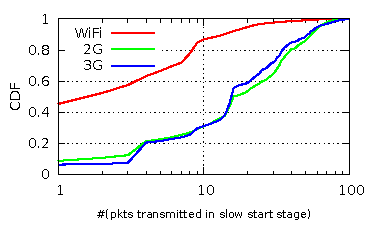
\includegraphics[width=0.8\linewidth]{web_slowstart_pkts}
\caption{Number of packets transmitted in slow start stage.}
\label{fig:web_ss_pkts}
\end{figure}

Figure~\ref{fig:web_ss_pkts} shows the distribution of packets which could be transmitted in slow start stage. In the figure, only these flows experiencing packet loss are considered. In the considered flows, flows in WiFi network could transmit less data packets in slow start stage than those in cellular network. This could be induced by higher packet loss rate in WiFi network, which we will investigate in Section~\ref{sec:web_pkt_loss}. In particular, 85\% of the considered flows (\ie 8.1\% of all flows) in WiFi network experience packet loss in the initial congestion window. This is an evidence that increasing initial congestion window to 10 segment size is not always helpful to all flows.

\subsubsection{Congestion Avoidance stage}

\begin{figure}[th]
\centering
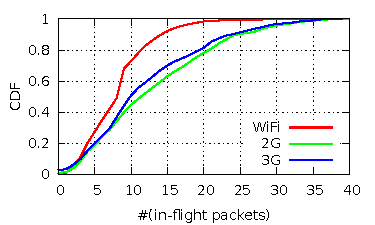
\includegraphics[width=0.8\linewidth]{web_ca_inflight}
\caption{Number of in flight packets when flows entering congestion avoidance stage.}
\label{fig:web_ca_inflight}
\end{figure}

Figure~\ref{fig:web_ca_inflight} shows the distribution of in flight packets when flows enter congestion avoidance stage. In the figure, only these flows experiencing packet loss are considered. In flight packets are those estimated in the network (\ie not dropped) yet not acknowledged by the receiver. When encountering packet loss, the number of in flight packets could be regarded as the number of packets allowed by network that could be transmitted in one RTT. In the figure, 80\% of flows in WiFi network have no more than 12 in flight packets. In contrast, 80\% of flows in cellular network have no more than 20 in flight packets. Flows in WiFi network have smaller in flight size than those in cellular network. This means that WiFi network allocates lower bandwidth for flows than cellular network.

\begin{figure}[th]
\centering
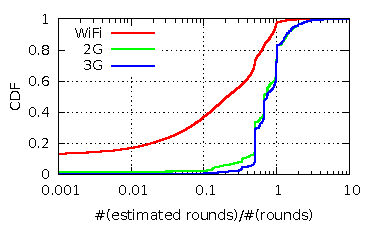
\includegraphics[width=0.8\linewidth]{web_ca_round}
\caption{The ratio of estimated rounds to practical rounds in congestion avoidance stage.}
\label{fig:web_ca_round}
\end{figure}

We use the number of in flight packets when encountering packet loss to approximate the ``allocated bandwidth'' to the flow. Thus, ideally the left data will be transmitted in $ceiling(\frac{\#(ca\_pkts)}{in\_flight})$ rounds (noted as $T_i$), where $ca\_pkts$ represents the packets transmitted in congestion avoidance stage, and $in\_flight$ is the number of in flight packets. Meanwhile, we could also calculate the practical rounds consumed to transmit the left data: $ceiling(\frac{ca\_time}{rtt})$ (noted as $T_p$), where $ca\_time$ is the time spent in congestion avoidance stage, and $rtt$ is the minimal RTT measured in the stage. We plot the ratio of the ideal rounds to the practical rounds (\ie $T_i/T_p$) in Figure~\ref{fig:web_ca_round}. When the ratio $T_i/T_p$ is close to 1, it means network allocates bandwidth similar to the estimated one. As the ratio is less than 1, it means network could only allocate less bandwidth less than the estimated one. 

From the figure, flows in the two access types behaves totally differently. In cellular network, 90\% of flows have the ratio value between 0.5 and 2, which demonstrates stability of bandwidth allocation in cellular network. Besides, 18\% of flows in cellular network have $T_i/T_p$ value larger than 1, which means those flows could ramp up the congestion window after packet loss. In contrast, nearly all flows in WiFi network have the $T_i/T_p$ value less than 1. Moreover, 18\% of flows in WiFi network have the ratio less than 0.01. This means once flows in WiFi network encounter packet loss, they could have more lost packets in the subsequent data transmission, which makes the number of in flight packets smaller.

\subsection{Impact of RTT}

\begin{figure}[th]
\centering
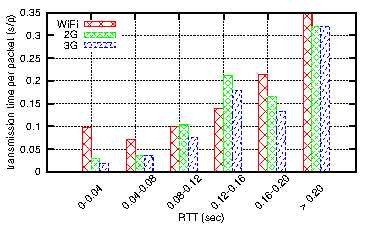
\includegraphics[width=0.8\linewidth]{web_rtt}
\caption{The average transmission time per packet under different RTT's.}
\label{fig:web_rtt}
\end{figure}

Here we investigate the impact of RTT on the transmission time per packet ($tpp$) of web search flows. We also use 0.4s interval to group the flows by their RTT's. The result is shown in Figure~\ref{fig:web_rtt}. From the figure, as the RTT value becomes larger, the overall $tpp$ grows correspondingly. For smaller RTT value (less than 0.08s), the $tpp$ value of flows in WiFi network is 1-4 times larger than that of flows in cellular network. When the RTT value is larger than 0.08s, flows in all networks have similar $tpp$ values. Note that most of flows (95\%) in cellular network have RTT smaller than 0.08s, which verifies that the $tpp$ value of flows in cellular is much lower than that of flows in WiFi network in Figure~\ref{fig:web_finish_time}.

\subsection{Impact of packet loss}
\label{sec:web_pkt_loss}

\begin{figure}[th]
\centering
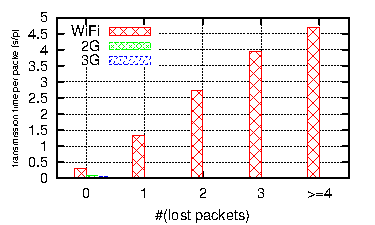
\includegraphics[width=0.8\linewidth]{web_loss_finish_time}
\caption{Transmission time per packet under different number of lost packets.}
\label{fig:web_loss_finish_time}
\end{figure}

Next, we investigate the impact of packet loss on the transmission time per packet ($tpp$). Note that the packet loss rate in 2G/3G network is less than 0.005\%, thus the impact in cellular network could be omitted. In contrast, about 5\% of flows in WiFi network encounter packet loss. Figure~\ref{fig:web_loss_finish_time} plots the $tpp$ values under different number of lost packets. In the figure, when there is no packet loss, the performance of each access type could be ranked as: 3G $>$ 2G $>>$ WiFi. In WiFi network, when the number of lost packets is larger than 3, the $tpp$ value is 15 times larger than that with no packet loss.

\subsection{Impact of timeout retransmission}

\begin{figure}[th]
\centering
	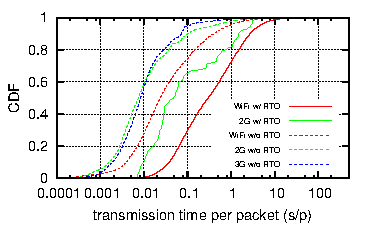
\includegraphics[width=0.8\linewidth]{web_timeout}
\caption{Transmission time per packet of flows with and without timeout retransmission.}
\label{fig:web_timeout}
\end{figure}

Even though flows in 2G network seldom encounters packet loss, 0.7\% of them suffer from timeout retransmission due to packet delay or lost acknowledgment. Figure~\ref{fig:web_timeout} shows the $tpp$ value of flows with and without timeout retransmission. In the figure, under the same access type (WiFi and 2G network), the $tpp$ value of flows with timeout retransmission is one order of magnitude larger than those without timeout retransmission. Considering flows with timeout retransmission, flows in 2G network have smaller $tpp$ value than those in WiFi network. The reasons are as follows. First, flows in 2G network have smaller RTT, and thus smaller RTO according to \cite{rfc62982011computing}. Second, many timeout retransmissions in 2G network are spurious due to packet delay or lost acknowledgment. When receiving Duplicate SACK if the first packet is not dropped, server recovers the original congestion window using F-RTO~\cite{sarolahti2005forward}, instead of increasing the window from 1 segment size.


\subsection{Summary of web search analysis}

The key observations on web search flows are summarized below.

\begin{itemize}
	\item Compared to the impact of RTT on voice recognition flow, RTT has limited affect on the transmission time per packet in web search.
	\item More than 50\% of flows spend 30\% of their total time on establishing connections.
	\item Flows in WiFi network are more likely to have lost packets, while flows in cellular network have more disordered packets.
	\item Even though 2G network has quite low packet loss rate (0.005\%), 0.7\% of flows encounter timeout retransmission, due to packet reordering.
\end{itemize}
